\documentclass[10pt, a4paper]{article}
% ===================== PACOTES =====================
\usepackage[brazil]{babel}
\usepackage[utf8]{inputenc}
\usepackage[T1]{fontenc}
\usepackage{geometry}
\geometry{a4paper, left=3cm, right=2cm, top=3cm, bottom=2.5cm}
\usepackage{graphicx}
\usepackage{indentfirst}
\usepackage{setspace}
\usepackage{hyperref}
\usepackage{caption}
\usepackage{subcaption}
\usepackage{amsmath}
\usepackage{enumitem}
\usepackage{parskip}
\usepackage[expansion=false]{microtype}
\usepackage{fancyhdr}
\usepackage{etoolbox}
\usepackage{listings}
\usepackage{xcolor}
\usepackage{courier}
\usepackage{mathpazo}               % Isso que dá a fonte legal

% ===================== ESTILO DOS BLOCOS DE CÓDIGO =====================
\definecolor{codebg}{RGB}{245,245,250}
\definecolor{darkgreen}{RGB}{0,100,0}
\definecolor{darkblue}{RGB}{0,0,160}

\lstset{
    language=R,
    basicstyle=\footnotesize\ttfamily,
    keywordstyle=\color{darkblue}\bfseries,
    commentstyle=\color{darkgreen}\itshape,
    stringstyle=\color{red},
    numberstyle=\scriptsize\color{gray},
    backgroundcolor=\color{codebg},
    numbers=none,
    breaklines=true,
    frame=single,
    rulecolor=\color{black!20},
    xleftmargin=12pt,
    xrightmargin=4pt,
    showstringspaces=false,
    tabsize=4,
    captionpos=b,
    abovecaptionskip=6pt,
    literate=
        {á}{{\'a}}1 {à}{{\`a}}1 {ã}{{\~a}}1 {â}{{\^a}}1
        {é}{{\'e}}1 {ê}{{\^e}}1 {í}{{\'i}}1
        {ó}{{\'o}}1 {õ}{{\~o}}1 {ô}{{\^o}}1
        {ú}{{\'u}}1 {ç}{{\c{c}}}1
}

% ===================== CONFIGURAÇÕES =====================
\setlength{\parindent}{1.25cm}
\setlength{\parskip}{0.4em}
\onehalfspacing

\hypersetup{
    colorlinks=true,
    linkcolor=blue,
    urlcolor=blue
}

\captionsetup{
    font=small,
    labelfont=bf
}

% ===================== CABEÇALHO E RODAPÉ =====================
\pagestyle{fancy}
\fancyhf{}
\renewcommand{\headrulewidth}{0.5pt}
\fancyhead[L]{%
    
\includegraphics[height=1cm]{imagens/ufc.png}
}
\fancyhead[R]{%
    \small{Homework 01 -- Estatística Descritiva}
}
\renewcommand{\footrulewidth}{0.5pt}
\fancyfoot[C]{\small Estatística para Engenharia}
\fancyfoot[R]{\small\thepage}
\setlength{\headheight}{30pt}
\fancypagestyle{empty}{
    \fancyhf{}
    \renewcommand{\headrulewidth}{0pt}
    \renewcommand{\footrulewidth}{0pt}
}

% ===================== DOCUMENTO =====================
\begin{document}

% ===================== CAPA =====================
\begin{titlepage}
\centering
\vspace*{2cm}

\includegraphics[width=0.35\textwidth]{imagens/ufc.png}\\[1.5cm]
{\Large\textbf{ESTATÍSTICA PARA ENGENHARIA}}\\[3cm]
{\large\textbf{HOMEWORK 01\\}
ANÁLISE DE COMPARTILHAMENTO DE BICICLETAS: UMA ABORDAGEM EM ESTATÍSTICA DESCRITIVA}\\[8cm]
\begin{flushleft}
\textbf{ALUNOS:}\\
ALEXANDRE DE AGUIAR MARTINS GRANGEIRO -- 578345\\
BRUNO DELUIZ LAGE -- 578342\\
DANNY SECUNDINO SOUSA FILHO -- 579763\\
SAULO GOMES PINTO -- 579493\\
\end{flushleft}
\end{titlepage}

\newpage

\section{Questão 1}
A primeira questão tem o objetivo de definir o escopo de dados
a serem utilizados pelo grupo ao longo de toda a análise. Para isso, 
foi feito um código R que fazia o que foi pedido no enunciado da questão.
O código é este:

\begin{lstlisting}
# =========================
# First Question
# =========================

# 1. Defining the highest student number
# students numbers
alexandre_sn <- 578345
bruno_sn <- 578342
danny_sn <- 579763
saulo_sn <- 579493

# highest student number
M <- max(c(alexandre_sn, bruno_sn, danny_sn, saulo_sn)) # 579763

# 2. Defining the start and the end of group's dataset
# start
r <- 1 + (M %% 100)     # 64

# end
end <- 300 + r - 1      # 363

# 3. Defining data_group (ie., the group's dataset)
# loading the entire file
all_data <- read.csv("HW1_bike_sharing.csv")

# defining our scope
data_group <- all_data[r:end, ]         # collect the lines 64-363

# 4. Defining the first 10 observations (we'll use them in the subsequent questions to validate our manual computations)
first_ten <- data_group[1:10, ]
\end{lstlisting}
É importante analisar o que, de fato, foi implemtentado com esse código:

Primeiramente, foram definidas variáveis \texttt{*\_sn} contendo, cada uma,
o valor do número de matrícula de um dos quatro integrantes do grupo. Os valores dos
números de matrículas são os seguintes:

\begin{enumerate}[label = \alph*)]
    \item Alexandre Grangeiro: 578345;
    \item Bruno Lage: 578342;
    \item Danny Secundino: 579763;
    \item Saulo Gomes: 579493.
\end{enumerate}

Após isso, a variável \texttt{M} foi declarada para guardar o maior número de matrícula dentre
os números de matrícula dos membros do grupo. Dessa forma, obtém-se

\[
\boxed{M = 579763}
\]

Com a informação do maior número de matrícula, foi pssível, então, definir o índice inicial do
subconjunto de dados a ser analisado nesse trabalho. Tal informação ficou guardada na variável
\texttt{r} e ele foi calculado da seguinte maneira:

\[
r = 1 + (M \; mod \; 100) = 1 + (579763 \; mod \; 100) = 1 + 63 \Rightarrow \boxed{r = 64}
\]

Em que $mod$ é a operação \textbf{resto de divisão}.\footnote{Em R, essa operação é realizada utilizando \texttt{\%\%}.}

Com o índice de início do conjunto de dados a ser analisado e considerando que tal conjunto deveria ter
300 elementos, também foi definido o fim:
\[
end = 300 + r - 1 = 300 + 64 - 1 \Rightarrow end = 363
\]

Com o início e o fim da janela que define o escopo das análises, foi declarado o \texttt{data\_group}, que pode ser usado
ao longo de todo o código para fazer as outras questões. Também foi definido o \texttt{first\_ten}, que contém as dez primeiras
observações do conjunto de dados do grupo e que será especialemente útil para comparar os cálculos que serão feitos manualmente com os que
serão obtidos com o código R.

Daí, foi possível coletar as datas da primeira e da última observação presentes em \texttt{data\_group}. Elas foram:
\begin{enumerate}[label = \alph*)]
    \item Data da primeira observação: 05/03/2011 (ou, no formato internacional, 2011-03-05)
    \item Data da última observação: 29/12/2011 (ou, no formato internacional, 2011-12-29) 
\end{enumerate}

Além disso, vale também apresentar as dez primeiras observações para que a análise ao longo do relatório seja melhor referenciada. Elas estão
dispostas na tabela a seguir:

\begin{table}[h]
\centering
\caption{Primeiras dez observações do conjunto \texttt{data\_group}}
\label{tab:first-ten}
\resizebox{\textwidth}{!}{%
\footnotesize
\begin{tabular}{ccccccccc}
\hline
\textbf{Instant} & \textbf{Data} & \textbf{Estação} & \textbf{Clima} & \textbf{Temp.} & \textbf{Casual} & \textbf{Registrados} & \textbf{Total} & \textbf{Baixa Utiliz.} \\
\hline
64 & 2011-03-05 & 1 & 2 & 15.8 & 640 & 1437 & 2077 & 0 \\
65 & 2011-03-06 & 1 & 2 & 15.4 & 114 & 491  & 605  & 1 \\
66 & 2011-03-07 & 1 & 1 & 10.7 & 244 & 1628 & 1872 & 1 \\
67 & 2011-03-08 & 1 & 1 & 12.0 & 316 & 1817 & 2133 & 0 \\
68 & 2011-03-09 & 1 & 2 & 12.1 & 191 & 1700 & 1891 & 0 \\
69 & 2011-03-10 & 1 & 3 & 16.0 & 46  & 577  & 623  & 1 \\
70 & 2011-03-11 & 1 & 2 & 13.0 & 247 & 1730 & 1977 & 0 \\
71 & 2011-03-12 & 1 & 1 & 13.5 & 724 & 1408 & 2132 & 0 \\
72 & 2011-03-13 & 1 & 1 & 15.8 & 982 & 1435 & 2417 & 0 \\
73 & 2011-03-14 & 1 & 1 & 13.3 & 359 & 1687 & 2046 & 0 \\
\hline
\end{tabular}%
}
\end{table}

As variáveis \texttt{total\_user} e \texttt{low\_usage} também foram incluídas na tabela, 
de modo a consolidar em uma única tabela todos os dados que serão utilizados ao longo das análises seguintes.

\textbf{Observação:} Aqui, foram postas as datas da primeira e da última observações, mas essa informação
também consta na saída do código fonte produzido. \textbf{Recomenda-se que se execute o código} \texttt{main.r} \textbf{para ver as informações
que são fornecidas na saída}.
\pagebreak

% ===================== QUESTÃO 2 =====================
\section{Questão 2}

O objetivo desta seção é caracterizar o conjunto de dados específico do grupo (\texttt{data\_group}), definido na Questão 1, calcular e interpretar as medidas de tendência central e os quartis das variáveis numéricas relevantes, identificar possíveis valores atípicos e definir a variável \texttt{low\_usage}. As análises foram realizadas inicialmente de forma manual, com as dez primeiras observações do conjunto (\texttt{first\_ten}), e, em seguida, verificadas e estendidas às 300 observações do grupo por meio do software R.

\subsection{Ponto 1 -- Caracterização das Variáveis}

\subsubsection{Classificação das variáveis}

\begin{itemize}
    \item \texttt{instant} -- Numérica (discreta): índice sequencial que identifica cada registro; assume valores inteiros que apenas ordenam as observações, sem magnitude física associada.
    \item \texttt{dteday} -- Categórica (ordinal): representa a data da observação; ainda que expressa em formato numérico (ano-mês-dia), não é submetida a operações aritméticas, apenas ordena os registros no tempo.
    \item \texttt{season} -- Categórica (nominal): codifica a estação do ano por meio de rótulos numéricos sem relação de ordem ou magnitude entre si.
    \item \texttt{weathersit} -- Categórica (ordinal): codifica a condição meteorológica; os códigos seguem uma ordem crescente de severidade do tempo.
    \item \texttt{temp} -- Numérica (contínua): representa a temperatura do dia, em graus Celsius; assume valores reais dentro de um intervalo contínuo.
    \item \texttt{casual} -- Numérica (discreta): representa a contagem diária de usuários casuais; assume apenas valores inteiros não negativos.
    \item \texttt{registered} -- Numérica (discreta): representa a contagem diária de usuários registrados; assume apenas valores inteiros não negativos.
    \item \texttt{total\_user} -- Numérica (discreta): variável derivada (\texttt{casual + registered}); representa o total diário de usuários do sistema.
\end{itemize}

\subsubsection{Categorias das variáveis categóricas}

\begin{itemize}
    \item \texttt{season}: 1 -- inverno, 2 -- primavera, 3 -- verão, 4 -- outono (estações do ano no hemisfério norte).
    \item \texttt{weathersit}: 1 -- céu limpo, 2 -- nublado, 3 -- chuva fraca, 4 -- chuva forte (ordenadas por severidade da condição meteorológica).
\end{itemize}

Cabe observar que, no subconjunto de 300 observações do grupo (\texttt{data\_group}), não há nenhum dia classificado com \texttt{weathersit = 4} (chuva forte), de modo que essa categoria, embora definida, não é representada na amostra analisada.

\subsubsection{Unidades e significado das variáveis numéricas}

\begin{itemize}
    \item \texttt{instant}: sem unidade de medida; identificador sequencial do registro.
    \item \texttt{temp}: graus Celsius; representa a temperatura observada no dia.
    \item \texttt{casual}: pessoas/dia; representa a quantidade de usuários que utilizaram o sistema sem vínculo de cadastro.
    \item \texttt{registered}: pessoas/dia; representa a quantidade de usuários cadastrados que utilizaram o sistema no mesmo dia.
    \item \texttt{total\_user}: pessoas/dia; variável derivada que soma \texttt{casual} e \texttt{registered}, representando o total de usuários do sistema em cada dia observado.
\end{itemize}

\subsubsection{Valores ausentes}
A verificação de valores ausentes foi feita por meio da função \texttt{is.na()} aplicada a \texttt{data\_group} (variável \texttt{has\_missing\_values} no código). O resultado obtido foi \texttt{FALSE}, isto é, não há valores ausentes em nenhuma das variáveis do conjunto de 300 observações do grupo.

\subsection{Ponto 2 -- Medidas de Tendência Central}

As medidas de tendência central foram calculadas para as variáveis numéricas relevantes (\texttt{temp}, \texttt{casual}, \texttt{registered} e \texttt{total\_user}): média, mediana e, quando aplicável, moda.

A média aritmética $\bar{x}$ é dada por
\[
\bar{x} = \frac{1}{n}\sum_{i=1}^{n} x_i
\]

A mediana $Me$ corresponde ao valor central do conjunto ordenado (ou à média dos dois valores centrais, quando $n$ é par):
\[
Me = \frac{x_{(n/2)} + x_{(n/2+1)}}{2}, \quad \text{para } n \text{ par}
\]

Para o cálculo manual, considera-se
\[
n = 10
\]

\subsubsection{Cálculo manual -- 10 primeiras observações}

A Tabela \ref{tab:valores-ordenados-10} apresenta os valores de cada variável ordenados de forma crescente, com os dois valores centrais (posições 5 e 6, usados no cálculo da mediana) destacados em negrito.

\begin{table}[h]
\centering
\caption{Valores ordenados (crescente) -- 10 primeiras observações}
\label{tab:valores-ordenados-10}
\begin{tabular}{ccccc}
\hline
\textbf{Posição} & \texttt{temp} (°C) & \texttt{casual} & \texttt{registered} & \texttt{total\_user} \\
\hline
1  & 10,7 & 46  & 491  & 605  \\
2  & 12,0 & 114 & 577  & 623  \\
3  & 12,1 & 191 & 1408 & 1872 \\
4  & 13,0 & 244 & 1435 & 1891 \\
5  & \textbf{13,3} & \textbf{247} & \textbf{1437} & \textbf{1977} \\
6  & \textbf{13,5} & \textbf{316} & \textbf{1628} & \textbf{2046} \\
7  & 15,4 & 359 & 1687 & 2077 \\
8  & 15,8 & 640 & 1700 & 2132 \\
9  & 15,8 & 724 & 1730 & 2133 \\
10 & 16,0 & 982 & 1817 & 2417 \\
\hline
\end{tabular}
\end{table}

\paragraph{\texttt{temp}}
\[
\begin{split}
\bar{x} &= \big(10{,}7+12{,}0+12{,}1+13{,}0+13{,}3 \\
&\quad{} +13{,}5+15{,}4+15{,}8+15{,}8+16{,}0\big)/10 \\
&= 137{,}6/10 = 13{,}76 \text{ °C}
\end{split}
\]
\[
Me = \frac{13{,}3 + 13{,}5}{2} = 13{,}40 \text{ °C}
\]

\paragraph{\texttt{casual}}
\[
\begin{split}
\bar{x} &= \big(46+114+191+244+247 \\
&\quad{} +316+359+640+724+982\big)/10 \\
&= 3863/10 = 386{,}30
\end{split}
\]
\[
Me = \frac{247 + 316}{2} = 281{,}50
\]

\paragraph{\texttt{registered}}
\[
\begin{split}
\bar{x} &= \big(491+577+1408+1435+1437 \\
&\quad{} +1628+1687+1700+1730+1817\big)/10 \\
&= 13910/10 = 1391{,}00
\end{split}
\]
\[
Me = \frac{1437 + 1628}{2} = 1532{,}50
\]

\paragraph{\texttt{total\_user}}
\[
\begin{split}
\bar{x} &= \big(605+623+1872+1891+1977 \\
&\quad{} +2046+2077+2132+2133+2417\big)/10 \\
&= 17773/10 = 1777{,}30
\end{split}
\]
\[
Me = \frac{1977 + 2046}{2} = 2011{,}50
\]

Os valores calculados manualmente coincidem com os obtidos por meio do código R (variáveis \texttt{xn\_first10\_*} e \texttt{me\_first10\_*}), conforme resumido na Tabela \ref{tab:tendencia-central-10}:

\begin{table}[h]
\centering
\caption{Medidas de tendência central -- 10 primeiras observações}
\label{tab:tendencia-central-10}
\begin{tabular}{lccc}
\hline
\textbf{Variável} & \textbf{Média} & \textbf{Mediana} & \textbf{Moda} \\
\hline
\texttt{temp}        & 13,76 °C & 13,40 °C & -- \\
\texttt{casual}      & 386,30   & 281,50   & -- \\
\texttt{registered}  & 1391,00  & 1532,50  & -- \\
\texttt{total\_user} & 1777,30  & 2011,50  & -- \\
\hline
\end{tabular}
\end{table}

Os mesmos cálculos foram estendidos às 300 observações do grupo (variáveis \texttt{xn\_*} e \texttt{me\_*}):

\begin{table}[h]
\centering
\caption{Medidas de tendência central -- 300 observações do grupo}
\label{tab:tendencia-central-300}
\begin{tabular}{lccc}
\hline
\textbf{Variável} & \textbf{Média} & \textbf{Mediana} & \textbf{Moda} \\
\hline
\texttt{temp}        & 22,11 °C & 22,20 °C & -- \\
\texttt{casual}      & 786,92   & 691,50   & -- \\
\texttt{registered}  & 3025,08  & 3238,50  & -- \\
\texttt{total\_user} & 3812,00  & 4067,50  & -- \\
\hline
\end{tabular}
\end{table}

Para nenhuma das quatro variáveis numéricas há um valor que se repita com frequência relevante, de modo que a moda não constitui uma medida significativa nesse conjunto de dados, tanto nas 10 primeiras observações quanto nas 300 observações do grupo.

Nas 300 observações, observa-se que a média de \texttt{casual} (786,92) é superior à sua mediana (691,50), indicando uma distribuição assimétrica à direita: a maioria dos dias apresenta uso casual moderado, enquanto um número menor de dias com uso muito elevado eleva o valor da média. Padrão semelhante, embora menos acentuado, é observado nas 10 primeiras observações. Já para \texttt{registered} e \texttt{total\_user}, a média é ligeiramente inferior à mediana, sugerindo leve assimetria à esquerda, compatível com a existência de alguns dias de uso registrado bastante baixo (possivelmente fins de semana ou feriados) que reduzem o valor médio. A variável \texttt{temp} apresenta média e mediana muito próximas nas 300 observações (22,11 °C e 22,20 °C), o que é coerente com o período coberto pela amostra do grupo, que se estende de março a dezembro de 2011, abrangendo estações de temperatura variada e resultando em uma distribuição aproximadamente simétrica.

\subsection{Ponto 3 -- Quartis e Valores Atípicos}

A variável escolhida para a análise de quartis e valores atípicos foi \texttt{casual} (número de usuários casuais por dia). A escolha se justifica por essa variável representar o quantitativo de usuários que utilizam o sistema de forma espontânea, sem vínculo de registro (\texttt{registered}). Por não estarem associados a um cadastro fixo, esses usuários refletem de maneira mais direta a demanda ocasional pelo serviço, tornando essa variável adequada para identificar dias com comportamento de uso atípico em relação ao padrão observado.

Os quartis $Q_1$, $Q_2$ e $Q_3$ dividem o conjunto ordenado de dados em quatro partes de igual tamanho. O intervalo interquartil é dado por
\[
IQR = Q_3 - Q_1
\]

Os limites inferior e superior para identificação de possíveis valores atípicos, segundo o critério do IQR, são dados por
\[
LI = Q_1 - 1{,}5 \cdot IQR \qquad LS = Q_3 + 1{,}5 \cdot IQR
\]

\subsubsection{Cálculo manual dos quartis -- 10 primeiras observações}

Para o cálculo manual, com $N = 10$, a posição de cada quartil no conjunto ordenado é obtida por
\[
\text{posição}(Q_1) = \frac{N+1}{4} = \frac{11}{4} = 2{,}75
\]
\[
\text{posição}(Q_2) = \frac{N+1}{2} = \frac{11}{2} = 5{,}50
\]
\[
\text{posição}(Q_3) = \frac{3(N+1)}{4} = \frac{33}{4} = 8{,}25
\]

Com os valores de \texttt{casual} já ordenados na Tabela \ref{tab:valores-ordenados-10} (46, 114, 191, 244, 247, 316, 359, 640, 724, 982), cada quartil é obtido por interpolação linear entre as posições inteiras adjacentes:
\[
Q_1 = 114 + 0{,}75 \cdot (191 - 114) = 171{,}75
\]
\[
Q_2 = 247 + 0{,}5 \cdot (316 - 247) = 281{,}50
\]
\[
Q_3 = 640 + 0{,}25 \cdot (724 - 640) = 661{,}00
\]
\[
IQR = Q_3 - Q_1 = 661{,}00 - 171{,}75 = 489{,}25
\]
\[
LI = 171{,}75 - 1{,}5 \cdot 489{,}25 = -562{,}125 \qquad LS = 661{,}00 + 1{,}5 \cdot 489{,}25 = 1394{,}875
\]

Como todos os valores de \texttt{casual} nas 10 primeiras observações estão contidos no intervalo $[-562{,}125;\,1394{,}875]$, nenhuma observação é classificada como atípica também pelo cálculo manual, resultado consistente com o obtido via R.

Para as 10 primeiras observações (variáveis \texttt{Q1\_f10}, \texttt{Q2\_f10}, \texttt{Q3\_f10}, \texttt{iqr\_f10}, \texttt{lower\_bound\_f10}, \texttt{upper\_bound\_f10} e \texttt{outliers\_f10} no código):

\begin{table}[h]
\centering
\caption{Quartis e limites de valores atípicos de \texttt{casual} -- 10 primeiras observações}
\label{tab:quartis-10}
\begin{tabular}{lc}
\hline
$Q_1$ & 204,25 \\
$Q_2$ & 281,50 \\
$Q_3$ & 569,75 \\
$IQR$ & 365,50 \\
Limite inferior & $-344{,}00$ \\
Limite superior & 1118,00 \\
\hline
\end{tabular}
\end{table}

Observa-se que os valores de $Q_1$ e $Q_3$ calculados manualmente ($171{,}75$ e $661{,}00$) diferem dos valores obtidos pela função \texttt{quantile()} do R ($204{,}25$ e $569{,}75$). Essa diferença decorre da convenção de interpolação adotada por cada método: o cálculo manual utiliza a posição $\frac{N+1}{4}$ (equivalente ao tipo 6 de quantil), enquanto a função \texttt{quantile()} do R utiliza, por padrão, a posição $1+(n-1)\cdot p$ (tipo 7). Já a mediana ($Q_2 = 281{,}50$) coincide exatamente entre os dois métodos, pois ambas as convenções resultam na mesma posição central ($\frac{N+1}{2} = 5{,}5$) para esse caso. Em ambos os métodos, entretanto, a conclusão quanto à ausência de valores atípicos nas 10 primeiras observações se mantém.

O mesmo procedimento (via R) foi aplicado às 300 observações do grupo (variáveis \texttt{Q1}, \texttt{Q2}, \texttt{Q3}, \texttt{iqr}, \texttt{lower\_bound}, \texttt{upper\_bound} e \texttt{outliers}):

\begin{table}[h]
\centering
\caption{Quartis e limites de valores atípicos de \texttt{casual} -- 300 observações do grupo}
\label{tab:quartis-300}
\begin{tabular}{lc}
\hline
$Q_1$ & 376,75 \\
$Q_2$ & 691,50 \\
$Q_3$ & 949,75 \\
$IQR$ & 573,00 \\
Limite inferior & $-482{,}75$ \\
Limite superior & 1809,25 \\
\hline
\end{tabular}
\end{table}

Nas 10 primeiras observações, nenhum dia foi classificado como valor atípico: todos os valores de \texttt{casual} nesse subconjunto encontram-se dentro do intervalo $[-344{,}00;\,1118{,}00]$. Já nas 300 observações do grupo, foram identificados 18 dias com valor de \texttt{casual} acima do limite superior (1809,25) -- não houve valores abaixo do limite inferior, o que é esperado, já que esse limite é negativo e \texttt{casual} não assume valores negativos. As datas classificadas como atípicas estão listadas na Tabela \ref{tab:outliers-300}.

\begin{table}[h]
\centering
\caption{Dias classificados como valores atípicos de \texttt{casual} -- 300 observações do grupo}
\label{tab:outliers-300}
\begin{tabular}{cc|cc}
\hline
\textbf{Data} & \textbf{\texttt{casual}} & \textbf{Data} & \textbf{\texttt{casual}} \\
\hline
30/04/2011 & 1965 & 09/07/2011 & 1988 \\
21/05/2011 & 2258 & 16/07/2011 & 2418 \\
28/05/2011 & 2001 & 17/07/2011 & 2006 \\
29/05/2011 & 2355 & 20/08/2011 & 1914 \\
04/06/2011 & 1869 & 03/09/2011 & 1935 \\
26/06/2011 & 1920 & 04/09/2011 & 2521 \\
02/07/2011 & 2204 & 08/10/2011 & 2235 \\
03/07/2011 & 2282 & 09/10/2011 & 2397 \\
04/07/2011 & 3065 & 15/10/2011 & 1899 \\
\hline
\end{tabular}
\end{table}

Observa-se que todas as datas atípicas se concentram entre final de abril e meados de outubro, período de clima mais ameno no hemisfério norte, e incluem finais de semana e datas próximas a feriados (como 04/07/2011, Dia da Independência dos EUA, e o final de semana de 28--29/05/2011, próximo ao feriado de Memorial Day). Esse padrão é coerente com a natureza da variável \texttt{casual}: por não exigir cadastro, o uso casual do sistema tende a ser mais sensível a condições favoráveis de lazer (bom tempo, folgas e feriados), o que explica a ocorrência de picos pontuais de demanda muito acima do padrão típico. Esses valores atípicos são relevantes para a análise do sistema por sinalizarem dias de pico de demanda que podem exigir redistribuição adicional de bicicletas ou reforço operacional.

\subsection{Ponto 4 -- Histograma e Boxplot}

Para a variável \texttt{casual}, foram construídos histogramas e boxplots, tanto para as 10 primeiras observações quanto para as 300 observações do grupo, permitindo analisar forma, dispersão, assimetria e a presença de valores atípicos.

\begin{figure}[h]
\centering
\begin{subfigure}{0.48\textwidth}
    \centering
    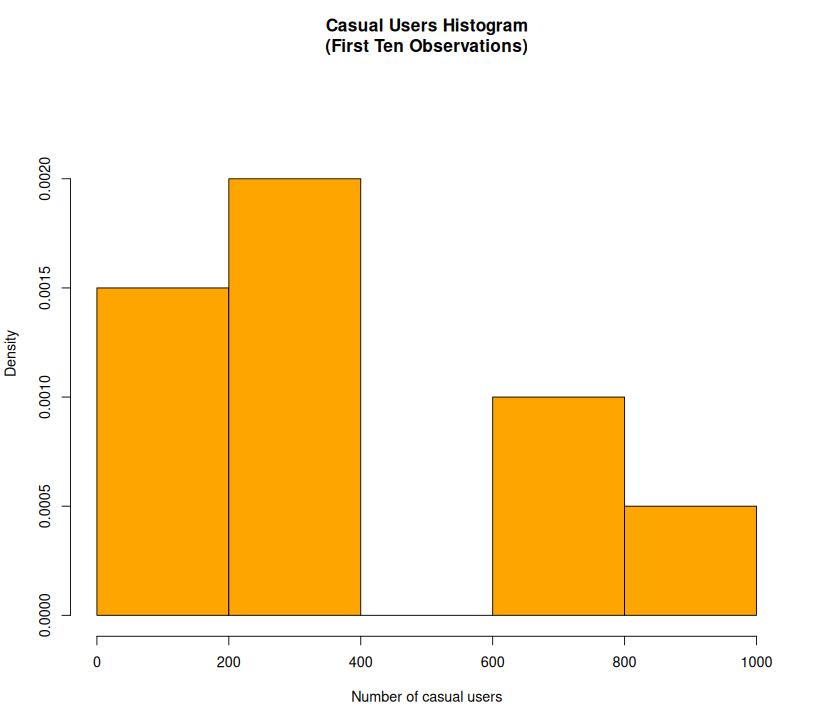
\includegraphics[width=\textwidth]{imagens/hist_casual_10obs.png}
    \caption{Histograma -- 10 primeiras observações}
    \label{fig:hist-casual-10}
\end{subfigure}
\hfill
\begin{subfigure}{0.48\textwidth}
    \centering
    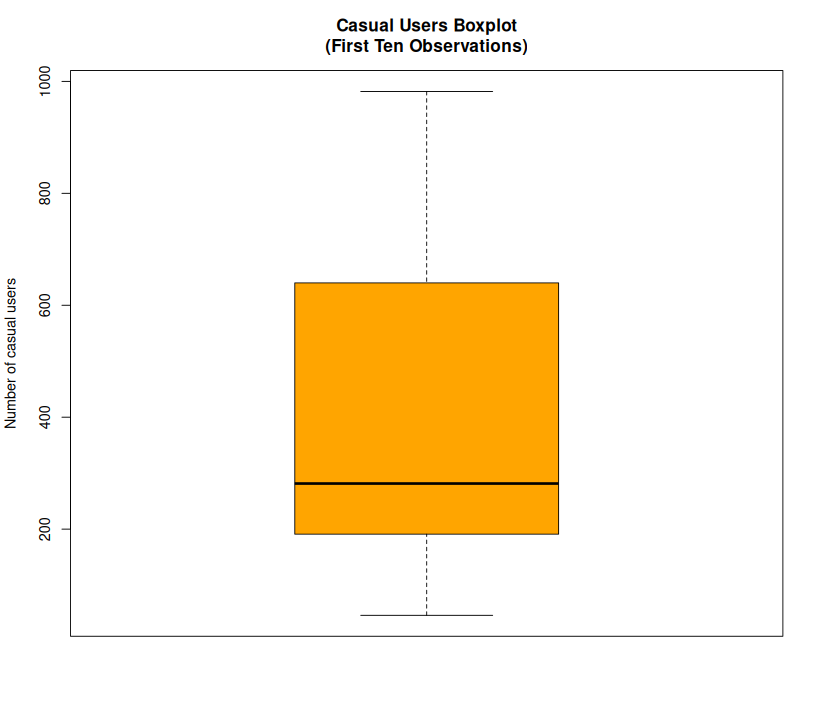
\includegraphics[width=\textwidth]{imagens/box_casual_10obs.png}
    \caption{Boxplot -- 10 primeiras observações}
    \label{fig:box-casual-10}
\end{subfigure}
\caption{Distribuição de \texttt{casual} -- 10 primeiras observações}
\label{fig:casual-10}
\end{figure}

\begin{figure}[h]
\centering
\begin{subfigure}{0.48\textwidth}
    \centering
    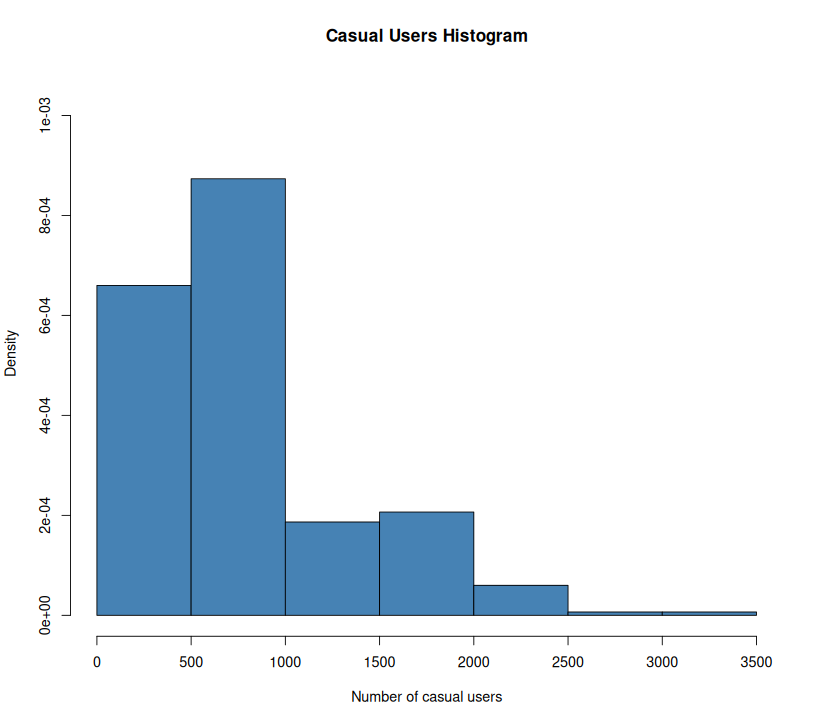
\includegraphics[width=\textwidth]{imagens/hist_casual_300obs.png}
    \caption{Histograma -- 300 observações do grupo}
    \label{fig:hist-casual-300}
\end{subfigure}
\hfill
\begin{subfigure}{0.48\textwidth}
    \centering
    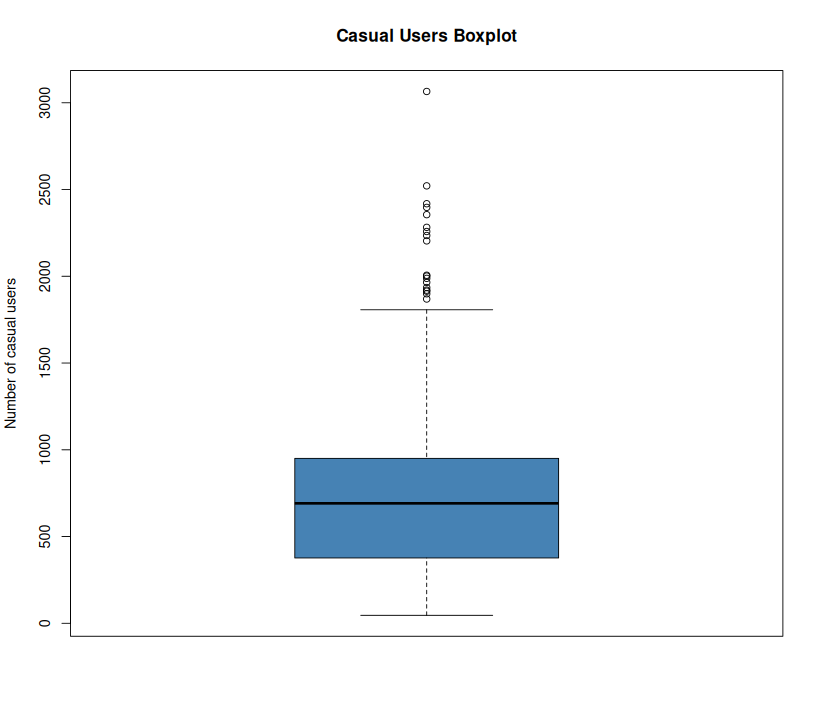
\includegraphics[width=\textwidth]{imagens/box_casual_300obs.png}
    \caption{Boxplot -- 300 observações do grupo}
    \label{fig:box-casual-300}
\end{subfigure}
\caption{Distribuição de \texttt{casual} -- 300 observações do grupo}
\label{fig:casual-300}
\end{figure}

Nas 10 primeiras observações, os valores de \texttt{casual} variam de 46 a 982 usuários por dia. O histograma exibe uma distribuição irregular, esperada dado o tamanho reduzido da amostra, com leve concentração nos valores mais baixos e uma cauda à direita. O boxplot correspondente não apresenta pontos além dos limites dos whiskers, em concordância com a ausência de valores atípicos apontada no Ponto 3, mas já evidencia uma mediana deslocada para a parte inferior da caixa, um primeiro indício de assimetria à direita.

Nas 300 observações do grupo, o histograma revela uma distribuição unimodal com assimetria positiva (à direita) bem mais evidente: a maior parte dos dias concentra-se na faixa entre aproximadamente 200 e 950 usuários casuais (intervalo entre $Q_1$ e $Q_3$), com uma cauda longa se estendendo até o valor máximo de 3065. O boxplot confirma esse padrão -- a mediana está deslocada para a parte inferior da caixa, o whisker superior é bem mais longo que o inferior, e os 18 valores atípicos aparecem representados como pontos isolados acima do limite superior. De forma geral, o histograma evidencia melhor a forma global da distribuição (concentração, cauda e multimodalidade, caso existisse), enquanto o boxplot evidencia de forma mais direta e quantitativa os quartis, a mediana e a posição exata dos valores atípicos.

\subsection{Ponto 5 -- Variável \texttt{low\_usage}}

Com base no primeiro quartil $Q_1$ de \texttt{total\_user}, foi definida a variável binária \texttt{low\_usage}, segundo o critério

\[
\text{low\_usage} =
\begin{cases}
1, & \text{se } \texttt{total\_user} < Q_1 \\
0, & \text{caso contrário}
\end{cases}
\]

Diferentemente da escolha de \texttt{casual} feita no Ponto 3 -- em que a variável foi selecionada pelo grupo entre as opções relevantes --, aqui a variável de referência é \texttt{total\_user} porque o próprio critério de definição de \texttt{low\_usage}, apresentado no enunciado, utiliza explicitamente o primeiro quartil dessa variável como limiar (Equação anterior).

\subsubsection{Cálculo manual de $Q_1$ -- 10 primeiras observações}

Assim como no Ponto 3, a posição do primeiro quartil no conjunto ordenado é obtida por
\[
\text{posição}(Q_1) = \frac{N+1}{4} = \frac{11}{4} = 2{,}75, \qquad N = 10
\]

Com os valores de \texttt{total\_user} já ordenados na Tabela \ref{tab:valores-ordenados-10} (605, 623, 1872, 1891, 1977, 2046, 2077, 2132, 2133, 2417), o quartil é obtido por interpolação linear entre a 2ª e a 3ª posições:
\[
Q_1 = 623 + 0{,}75 \cdot (1872 - 623) = 1559{,}75
\]

Esse valor difere do obtido pela função \texttt{quantile()} do R ($Q_1 = 1876{,}75$) pela mesma razão discutida no Ponto 3: a convenção de interpolação da posição $\frac{N+1}{4}$ (tipo 6) diverge da convenção padrão do R, $1+(n-1)\cdot p$ (tipo 7). Usando o valor manual ($1559{,}75$), apenas 2 das 10 primeiras observações seriam classificadas como \texttt{low\_usage} (20\%), contra as 3 observações (30\%) obtidas com o valor verificado em R. Os resultados apresentados a seguir seguem o valor calculado via R, em consonância com a metodologia adotada no restante do relatório.

Para as 10 primeiras observações, o valor de referência foi $Q_1 = 1876{,}75$ (variável \texttt{Q1\_lowusage\_f10}), resultando em 3 dias classificados como de baixa utilização, correspondendo a uma proporção de 30\% (variável \texttt{prop\_lu\_f10}).

Para as 300 observações do grupo, o valor de referência foi $Q_1 = 3116{,}50$ (variável \texttt{Q1\_lowusage}), resultando em 75 dias classificados como de baixa utilização, correspondendo a uma proporção de 25\% (variável \texttt{prop\_lu}).

Por construção, a proporção de dias classificados como \texttt{low\_usage} tende a se aproximar de 25\%, já que o critério utiliza exatamente o primeiro quartil da própria distribuição de \texttt{total\_user} -- o que é confirmado pelo resultado obtido nas 300 observações do grupo. Na amostra reduzida de 10 observações, a proporção observada (30\%) se afasta ligeiramente desse valor teórico em razão do tamanho pequeno da amostra, que torna a posição exata do quartil mais sensível a poucos valores e a possíveis empates. No contexto do sistema, os dias marcados como \texttt{low\_usage} correspondem tipicamente a condições que desestimulam o uso das bicicletas -- como baixas temperaturas, condições meteorológicas desfavoráveis ou dias da semana com menor mobilidade --, constituindo uma variável útil para segmentar e investigar os fatores associados à baixa demanda do sistema.

\section{Questão 3}
\section{Questão 4}

\end{document}